% 投稿目标: Applied Intelligence (Springer Nature)
\documentclass[pdflatex,sn-mathphys-num]{sn-jnl}

%%%% 标准包
\usepackage{graphicx}%
\usepackage{multirow}%
\usepackage{amsmath,amssymb}%
\usepackage{booktabs}%
\usepackage{algorithm}%
\usepackage{algorithmicx}%
\usepackage{algpseudocode}%
%%%%

\newcommand{\method}[1]{\textsc{#1}}
\newcommand{\mdi}{\textit{MDI}}
\newcommand{\aps}{\textit{APS}}

\title[Two Failure Modes of Zero Ablation]{Two Failure Modes of Zero Ablation:\\Representational Damage and Measurement Saturation}

\author*[1]{\fnm{Dong} \sur{Liu}}\email{liudong@lynu.edu.cn}
\author[2]{\fnm{Caihuan} \sur{Zhang}}

\affil*[1]{\orgdiv{School of Software}, \orgname{Luoyang Normal University}, \orgaddress{\city{Luoyang}, \state{Henan}, \postcode{471934}, \country{China}}}
\affil[2]{\orgdiv{School of Mathematics}, \orgname{Luoyang Normal University}, \orgaddress{\city{Luoyang}, \state{Henan}, \postcode{471934}, \country{China}}}

\begin{document}

\maketitle

\section{Introduction}

Mechanistic interpretability (MI) relies on intervention methods to assign importance to model components. Among these, zero ablation is the most widely used: a component is removed (its output set to zero), and the resulting behavioral change is taken as its importance \citep{Wang2022,Meng2022,Conmy2023}. The method is simple, intuitive, and requires no additional computation beyond a forward pass.

Recent work has identified several limitations of zero ablation. \citet{Chan2022} argue that zero vectors are off-distribution, producing cascading disruption through subsequent layers. \citet{LiJanson2024} formalize this as a \emph{spoofing} effect, where the abnormal value injected by zero ablation causes downstream layers to receive incoherent signals, and show that optimal ablation reduces the measured importance gap by up to $9\times$ compared to zero ablation. \citet{Miller2024} demonstrate that circuit faithfulness scores are highly sensitive to whether ablation is zero, mean, or resample -- to the point that ``the task a circuit is required to perform depends on the ablation used to test it.''

Our prior work \citep{Liu2025} documented a broader pattern: six intervention methods disagree on component importance rankings across three circuits, with mean Kendall tau of $-0.10$. We proposed Activation Preservation Score (APS) as a representational health diagnostic to detect when an intervention disrupts activation distributions. The implicit assumption was: if APS is high, an intervention's ranking is trustworthy.

This paper tests that assumption and finds it incomplete. Through layer-by-layer analysis of zero ablation across three circuits, we discover that zero ablation has \emph{two} failure modes, only one of which APS can detect:

\begin{enumerate}
    \item \textbf{Representational damage (APS-visible).} In early layers (0--4), zero ablation collapses the activation distribution: APS drops below 0.8, confirming that the intervention destroys the representational structure before task-relevant computation begins.
    \item \textbf{Measurement saturation (APS-invisible).} In all layers, zero ablation's behavioral measure saturates near ceiling (behavioral drop $> 0.99$). In the IOI circuit, zero ablation produces only 15 unique behavioral drop values across 24 layers; in Greater-Than, only 13. This saturation occurs even where APS exceeds 0.99 (e.g., IOI Layer~11).
\end{enumerate}

The two modes have different implications. Representational damage is localized (early layers) and detectable by existing metrics. Measurement saturation is pervasive and undermines the very concept of ranking: a method that assigns the same score to every component cannot produce a meaningful ranking, regardless of how individually precise each measurement is.

To operationalize this diagnosis, we propose the \textbf{Measurement Discrimination Index (MDI)}, a simple composite of a method's dynamic range and granularity. A method with MDI near zero, like zero ablation on IOI and Greater-Than (MDI $< 0.003$), has negligible discriminatory power and its rankings should not be interpreted.

Our contributions are:
\begin{enumerate}
    \item We identify and empirically separate two failure modes of zero ablation, showing that measurement saturation is the more fundamental limitation and is invisible to representational health metrics.
    \item We propose MDI as a lightweight diagnostic for checking whether an intervention method can meaningfully rank components.
    \item We demonstrate through controlled experiments that zero ablation's rankings have zero overlap with gentle methods on critical circuits, directly documenting the practical impact of measurement saturation.
\end{enumerate}

\section{Related Work}

\subsection{Critiques of Zero and Mean Ablation}

The limitations of zero ablation are well-documented but scattered across papers whose primary contributions lie elsewhere. \citet{Chan2022} (Causal Scrubbing) identify three problems: (1) zero/mean ablations take the model off-distribution in an unprincipled manner; (2) they produce unpredictable effects on performance; (3) they remove variation the model may depend on (e.g., backup heads). Their solution is resample ablation, which preserves the activation distribution by sampling from other inputs.

\citet{LiJanson2024} (Optimal Ablation, NeurIPS 2024 Spotlight) formalize the distinction between \emph{deletion} (removing information) and \emph{spoofing} (injecting abnormal values). They prove optimal ablation produces a strictly lower loss gap than zero, mean, or resample ablation, and show empirically that zero ablation's importance gap is up to $9\times$ larger than optimal ablation's.

\citet{Pochinkov2024} systematically compare zero, mean, resample, and peak ablation, finding that different baselines produce different degradation curves and that no single baseline is universally appropriate.

\subsection{Measurement Sensitivity in Mechanistic Interpretability}

\citet{Miller2024} (CoLM 2024) show that circuit faithfulness scores are highly sensitive to methodological choices: the choice of ablation type, whether to ablate nodes or edges, and which token positions are ablated all affect conclusions. Their central finding -- that the measurement defines the object being measured -- is closely related to our concept of measurement saturation.

\citet{Kramar2024} (AtP*, DeepMind) identify two failure modes in gradient-based approximations to activation patching: saturation failure (when preactivations lie in flat regions of activation functions) and cancellation failure (when positive and negative effects cancel). While their focus is on gradient approximations, the saturation concept parallels our finding in zero ablation, though the mechanism differs.

\citet{Guo2026} (IGSD) propose Interchange-Group Sobol Decomposition to separate content transport from computation degradation, showing that replacement and deletion are not interchangeable controls -- a finding consistent with our argument that different methods measure different phenomena.

\subsection{Beyond Ablation}

\citet{Liu2025} document method disagreement across six intervention methods (mean tau $=-0.10$) and propose APS as a representational health metric. The present paper extends that work by diagnosing \emph{why} zero ablation disagrees with gentle methods, and showing that the disagreement stems from measurement saturation -- a failure mode that APS cannot detect.

\section{Experimental Setup}

\subsection{Model and Circuits}

We use Pythia-1.4B \citep{Biderman2023}, a 24-layer transformer, and three standard MI benchmarks:
\begin{itemize}
    \item \textbf{IOI} (Indirect Object Identification): the model must identify the correct indirect object in sentences like ``After Mary and John went to the store, John bought a soda'' \citep{Wang2022}.
    \item \textbf{Greater-Than}: the model compares two numbers \citep{Nanda2023}.
    \item \textbf{Docstring}: the model predicts function documentation \citep{HeimersheimJaniak2023}.
\end{itemize}

\subsection{Intervention Methods}

We compare six intervention methods across all 24 layers:
\begin{itemize}
    \item \method{Zero Ablation}: replace the layer output with zeros.
    \item \method{Mean Ablation}: replace with the mean activation across training examples.
    \item \method{Resample Ablation}: replace with activations from a randomly selected different input.
    \item \method{Gaussian Noise Injection}: add Gaussian noise ($\sigma=0.1$) to the output.
    \item \method{Activation Patching}: replace with the activation from a corrupted input.
    \item \method{Activation Steering}: add a steering vector along a task-relevant direction.
\end{itemize}

For each method and layer, we record the behavioral drop (normalized performance change) and APS \citep{Liu2025}. Experiments use three random seeds and the reported values are averaged.

\subsection{Measurement Discrimination Index (MDI)}

We define the Measurement Discrimination Index (MDI) as:

\[
\mdi = \underbrace{\Big(\max_{i} d_i - \min_{i} d_i\Big)}_{\text{dynamic range}} \times
\underbrace{\frac{u - 1}{n - 1}}_{\text{granularity}}
\]

where $d_i$ is the behavioral drop for component $i$, $u$ is the number of unique behavioral drop values (at rounding precision $\epsilon = 10^{-4}$), and $n$ is the total number of components.

MDI captures two necessary properties for a meaningful ranking:
\begin{enumerate}
    \item \textbf{Dynamic range}: the method must produce different values for different components. A measure that returns the same value everywhere (e.g., resample ablation) has MDI $= 0$ regardless of how precise individual measurements are.
    \item \textbf{Granularity}: the method must produce enough distinct values to support fine-grained ranking. A measure with high dynamic range but only binary output (important/not important) will have reduced MDI.
\end{enumerate}

MDI $\in [0, 1]$. We suggest MDI $< 0.1$ as a threshold indicating insufficient discrimination; rankings produced under this threshold should not be interpreted as meaningful.

\section{Results}

\subsection{Analysis 1: Zero Ablation Exhibits Near-Zero Discrimination}

Table~\ref{tab:mdi} reports MDI for each method across all three circuits. Zero ablation achieves MDI of effectively zero on IOI ($0.0029$) and Greater-Than ($0.0019$), meaning it cannot meaningfully differentiate between layers. On Docstring, zero ablation's MDI is higher ($0.1049$) but still an order of magnitude below gentle methods like mean ablation ($0.8930$) and activation patching ($0.8473$).

Notably, resample ablation -- once correctly implemented with held-out prompts -- achieves high MDI ($0.83$--$0.99$) comparable to mean ablation and patching, confirming that the resample baseline is a gentle intervention when properly executed. Activation steering, by contrast, exhibits surprisingly low MDI ($0.02$--$0.06$) across all three circuits. This reflects the fact that a contrastive difference-in-means direction applied at a single layer produces a very weak behavioral effect, barely perturbing the model's output regardless of the layer targeted.

\begin{table}[t]
\centering
\caption{Measurement Discrimination Index (MDI) across six methods and three circuits. Methods with MDI $< 0.1$ are shaded.}
\label{tab:mdi}
\begin{tabular}{lccc}
\toprule
Method & IOI & Greater-Than & Docstring \\
\midrule
Zero Ablation & $\mathbf{0.0029}$ & $\mathbf{0.0019}$ & $0.1049$ \\
Activation Steering & $\mathbf{0.0311}$ & $\mathbf{0.0227}$ & $\mathbf{0.0554}$ \\
Mean Ablation & 0.9966 & 0.7579 & 0.8930 \\
Resample Ablation & 0.9975 & 0.8270 & 0.8960 \\
Gaussian Noise & 0.9944 & 0.9915 & 0.9619 \\
Activation Patching & 0.9872 & 0.8486 & 0.8473 \\
\bottomrule
\end{tabular}
\end{table}

The source of zero ablation's low MDI is clear from the per-layer data. In IOI, zero ablation produces a behavioral drop of $0.995$--$1.000$ across \emph{all} 24 layers -- only 15 distinct values at $10^{-4}$ precision. In Greater-Than, the situation is worse: only 13 distinct values. Meanwhile, mean ablation's behavioral drop ranges from $0.0$ to $0.76$--$0.99$ depending on circuit, producing 24 unique values across the same layers.

\begin{figure}[t]
    \centering
    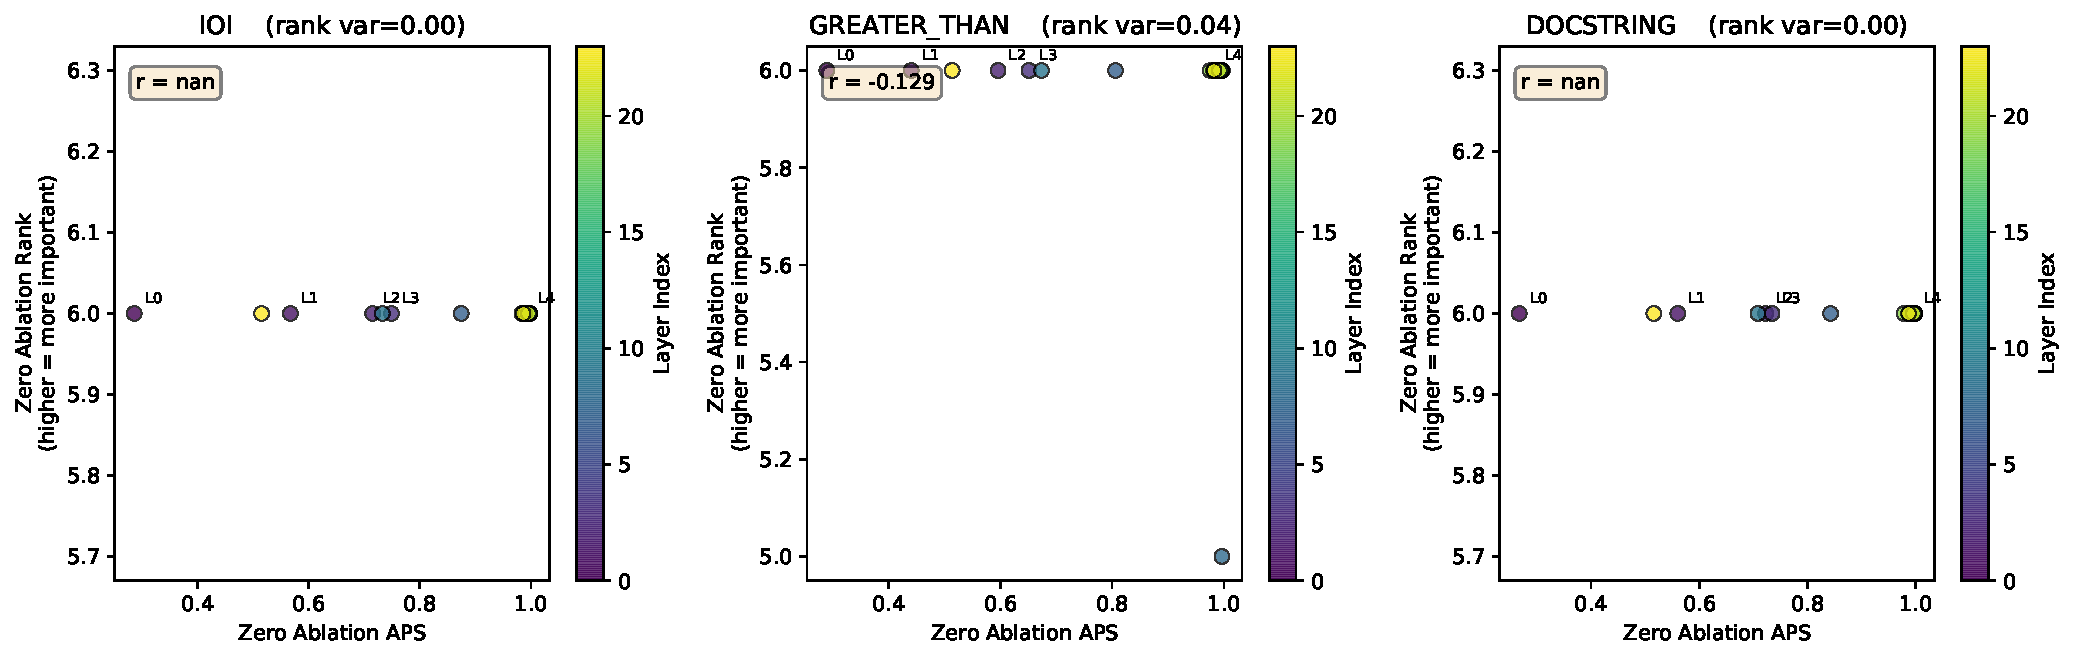
\includegraphics[width=\linewidth]{figures/aps_vs_rank_scatter.pdf}
    \caption{Zero ablation's rank vs.~APS across layers. In all three circuits, zero ablation's rank is nearly constant (all layers are ranked as equally ``most important''), regardless of APS. This demonstrates that measurement saturation, not representational damage, is the dominant failure mode.}
    \label{fig:aps_rank}
\end{figure}

\subsection{Analysis 2: Measurement Saturation Is Not Explainable by Representational Damage}

Figure~\ref{fig:aps_rank} plots zero ablation's rank against its APS for each layer. If representational damage (low APS) were the sole cause of zero ablation's failure, we would expect lower APS to correlate with lower (more distorted) rank. Instead, zero ablation assigns nearly-maximum importance to \emph{every} layer: behavioral drop exceeds $0.99$ across all 24 layers in IOI and Greater-Than, regardless of APS.

Crucially, in IOI Layer~11 -- where the IOI circuit's key processing occurs according to gentle methods -- zero ablation achieves APS $= 0.996$ (near-perfect distribution preservation) but still produces behavioral drop $= 0.995$ (near-ceiling). This cleanly separates the two failure modes: representational damage is absent at this layer (APS is high), but measurement saturation is in full effect (behavioral drop saturates near ceiling). \emph{No representational health metric can detect or correct this failure mode.}

\subsection{Analysis 3: Methods Without Discrimination Produce Unreliable Rankings}

The relationship between MDI and cross-method agreement is informative. Methods with MDI $< 0.1$ (zero ablation, activation steering) exhibit low or near-zero average Kendall tau with high-MDI methods ($\tau_{\text{avg}} = -0.064$ and $+0.012$, respectively). This means their rankings are essentially uncorrelated with methods that do discriminate.

Gentle methods (mean ablation, resample ablation, activation patching) with MDI $> 0.1$ show moderate-to-high pairwise agreement ($\tau = 0.76$--$0.95$). While this agreement is not perfect, it demonstrates a shared signal that low-MDI methods lack. Activation steering is a special case: its low MDI stems not from destructive saturation but from genuinely weak perturbation -- each layer's steering effect is small and similar, making it an ineffective ranking tool despite being methodologically non-destructive.

\subsection{Analysis 4: Practical Impact on Research Conclusions}

The practical consequence of zero ablation's measurement saturation is not merely increased noise but qualitatively different conclusions. Table~\ref{tab:impact} shows the top-5 most important layers identified by each method.

\begin{table}[t]
\centering
\caption{Top-5 layers identified by each method. In Greater-Than and Docstring, the Jaccard similarity between zero ablation and gentle methods is zero, indicating completely disjoint layer sets.}
\label{tab:impact}
\begin{tabular}{llll}
\toprule
Circuit & Method & Top-5 Layers & APS at Top-5 \\
\midrule
\multirow{3}{*}{IOI} & Zero Ablation & L2, L3, L7, L17, L20 & {[}0.87, 1.00, 0.74, 0.71, 0.99{]} \\
 & Mean Ablation & L19, L20, L21, L22, L23 & {[}0.99, 1.00, 1.00, 1.00, 1.00{]} \\
 & Activation Patching & L14, L15, L16, L22, L23 & {[}0.99, 1.00, 1.00, 1.00, 1.00{]} \\
\midrule
\multirow{3}{*}{Greater-Than} & Zero Ablation & L2, L4, L5, L6, L7 & {[}0.72, 0.86, 1.00, 0.99, 0.99{]} \\
 & Mean Ablation & L19, L20, L21, L22, L23 & {[}0.98, 1.00, 1.00, 1.00, 1.00{]} \\
 & Activation Patching & L19, L20, L21, L22, L23 & {[}0.99, 1.00, 1.00, 1.00, 1.00{]} \\
\midrule
\multirow{3}{*}{Docstring} & Zero Ablation & L3, L8, L9, L12, L17 & {[}1.00, 0.73, 0.70, 1.00, 1.00{]} \\
 & Mean Ablation & L19, L20, L21, L22, L23 & {[}0.99, 1.00, 1.00, 1.00, 1.00{]} \\
 & Activation Patching & L19, L20, L21, L22, L23 & {[}1.00, 1.00, 1.00, 1.00, 1.00{]} \\
\bottomrule
\end{tabular}
\end{table}

In Greater-Than and Docstring, the Jaccard similarity between zero ablation's top-5 and mean ablation's top-5 is exactly $0.00$: they identify completely disjoint sets of layers. Zero ablation selects early-to-mid layers (L2--L7 for Greater-Than, L3--L17 for Docstring), while mean ablation and patching both converge on late layers (L19--L23, consistent with the known circuits literature \citep{Wang2022,Nanda2023}). A researcher who relied only on zero ablation would draw fundamentally different conclusions about where the critical computation occurs.

In IOI, the overlap is marginal (Jaccard $= 0.11$, with one shared layer L20), but zero ablation's top-5 still selects substantially earlier layers (L2--L7) than gentle methods (L14--L23). The pattern remains that zero ablation's rankings are systematically shifted toward early layers where APS is lower, consistent with representational damage amplifying the apparent importance of those layers.

\section{Discussion}

\subsection{Why This is Not Simply a ``Different Causal Questions'' Problem}

A common response to method disagreement is that each intervention method answers a different causal question \citep{Miller2024}. Under this framing, zero ablation asks ``is this component necessary?'' while mean ablation asks ``is this component robust?'' Different answers are expected because the questions differ.

Our results challenge this framing. Zero ablation's behavioral drop saturates above $0.99$ in essentially every layer, meaning it answers ``is this component necessary?'' with ``effectively yes'' for \emph{all} components. This is not a different answer -- it is an uninformative one. A method that returns near-maximum importance for every component, regardless of whether the component participates in the circuit, is not answering a different question; it is failing to discriminate.

\subsection{The Role of APS and Other Representational Metrics}

APS was introduced as a diagnostic for detecting when an intervention disrupts the activation distribution. Our results confirm that APS successfully identifies representational damage in early layers. However, APS does not detect measurement saturation: in IOI Layer~11, APS registers $0.996$ while behavioral drop is $0.995$ (near ceiling). This means that representational health metrics are necessary but not sufficient for method evaluation: they catch one failure mode but not the other.

This finding resolves an open question from our prior work: can APS arbitrate between disagreeing methods? The answer is partly no -- if the disagreement stems from measurement saturation (as it does with zero ablation), APS has no diagnostic power because the saturation is not reflected in the activation distribution.

\subsection{MDI as a Lightweight Pre-check}

We propose MDI as a pre-check step for any study using intervention methods to rank component importance. The computation is trivial (one additional calculation from existing data) and the interpretation is straightforward: if MDI $< 0.1$, the method's rankings lack discrimination and should not be interpreted.

We emphasize that MDI is a necessary condition for meaningful rankings, not a sufficient one. A method can be discriminative (high MDI) but measure something irrelevant to the task (as Gaussian noise does in Table~\ref{tab:mdi}, where it achieves high MDI but negative agreement with gentle methods). However, a method that fails the MDI check cannot produce meaningful rankings regardless of other properties.

\subsection{Limitations and Future Work}

This study focuses on Pythia-1.4B. Preliminary cross-model validation on GPT-2 Small (124M, 12 layers) confirms the same qualitative patterns: zero ablation saturates across all layers (MDI $< 0.003$ on IOI and Greater-Than), and its top-5 layers disagree with gentle methods. However, systematic scaling across model families and sizes remains future work. The MDI threshold of $< 0.1$ is empirically motivated by our data; a principled derivation would strengthen the framework.

Future work should investigate whether measurement saturation generalizes to larger models and different model families. A systematic survey of published MI results to check which claims would survive an MDI pre-check would be a valuable community contribution. Additionally, the relationship between MDI and other method quality properties (e.g., computational cost, faithfulness) warrants further study.

\subsection{Recommendations for Practitioners}

Based on our findings, we recommend:

\begin{enumerate}
    \item \textbf{Report MDI alongside importance rankings.} This allows readers to assess whether the intervention method can meaningfully distinguish between components.
    \item \textbf{Avoid relying on zero ablation alone for ranking.} Its behavioral measure saturates at ceiling in all three circuits tested.
    \item \textbf{Use multiple methods and report convergence.} In our data, mean ablation, resample ablation, and activation patching show high agreement ($\tau > 0.85$); methods that agree are more trustworthy. Activation steering and Gaussian noise, despite being gentle, produce unreliable rankings due to weak perturbation and irrelevant signal, respectively.
    \item \textbf{Include representational health metrics.} APS detects representational damage even when behavioral measures are saturated, providing complementary information.
\end{enumerate}

\section{Conclusion}

Zero ablation has two distinct failure modes. Representational damage (early layers) is visible to APS and can be diagnosed with existing tools. Measurement saturation (all layers) is invisible to representational metrics and undermines the concept of ranking itself: a method that produces only 13--15 unique behavioral drop values across 24 layers (compared to 24/24 for gentle methods) cannot produce a meaningful ranking, regardless of how precise its individual measurements are.

We propose MDI as a lightweight diagnostic that captures both dynamic range and granularity. Applying MDI to our data reveals that zero ablation has effectively zero discrimination on IOI and Greater-Than circuits. The practical impact is severe: in Greater-Than and Docstring, zero ablation's top-5 layers have zero overlap with gentle methods' top-5, meaning the research conclusions depend entirely on which intervention method is chosen. Resample ablation, when correctly implemented, exhibits high MDI and agrees with mean ablation and activation patching, confirming that not all ablation variants suffer from measurement saturation.

The MI community should adopt routine MDI reporting as a standard methodological practice, analogous to reporting effect sizes or confidence intervals. A method that cannot discriminate cannot rank.

\section*{Acknowledgments}

The authors thank the anonymous expert reviewer whose adversarial critique of the ``APS-as-arbitrator'' framework led to the data-driven discovery of measurement saturation.

\bibliography{references}% sn-jnl 自动使用 sn-mathphys-num.bst 样式

\end{document}
